\documentclass{standalone}
\usepackage{tikz}
\usetikzlibrary{patterns, positioning}


\begin{document}
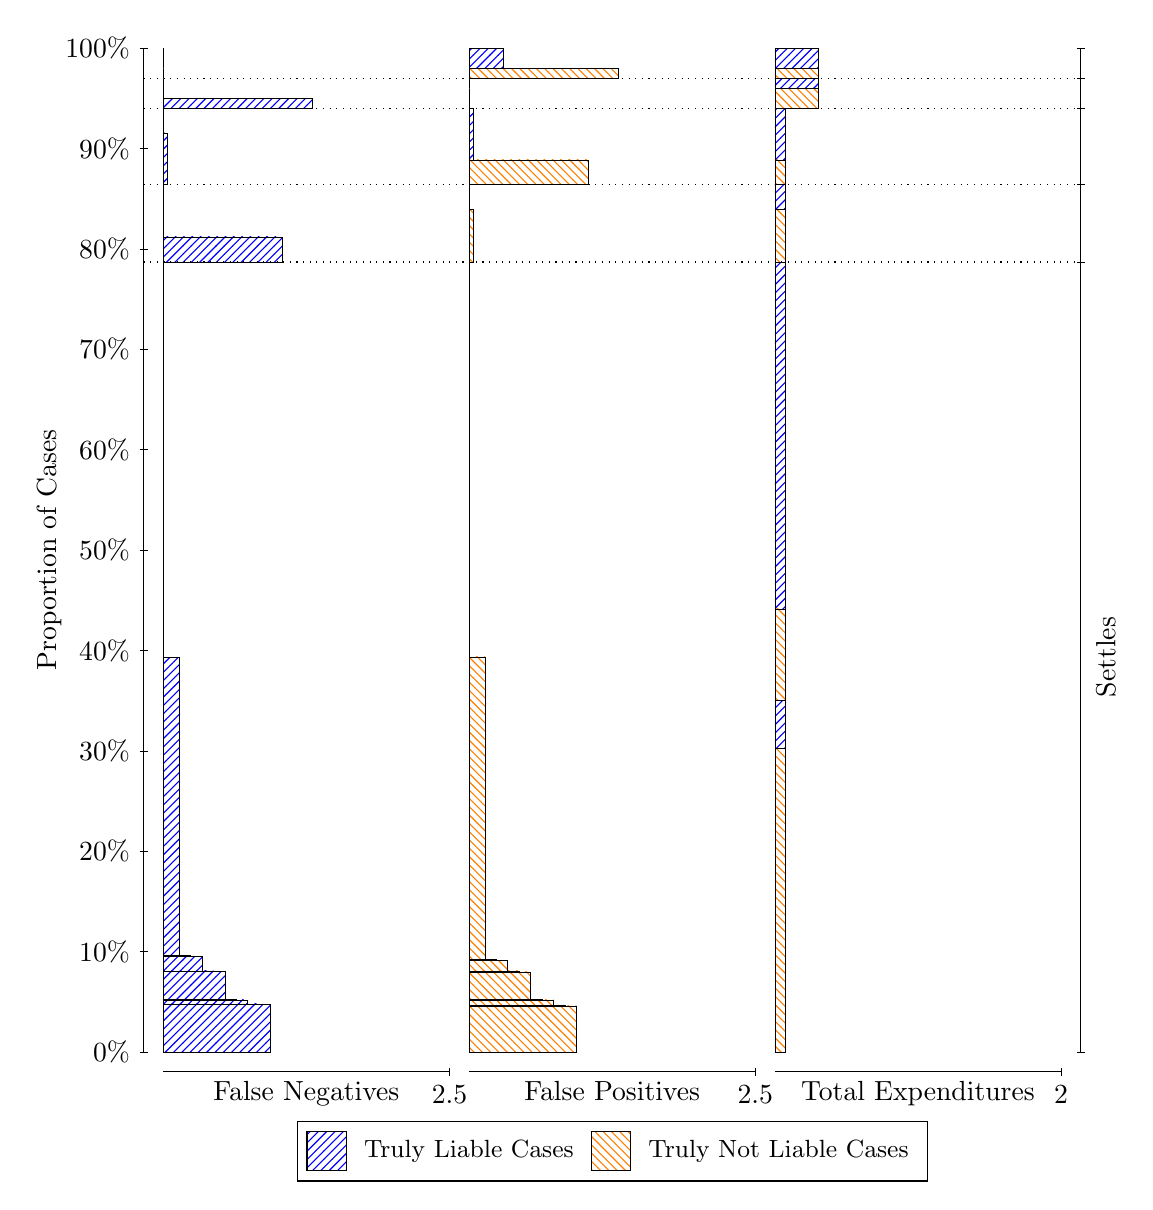
\begin{tikzpicture}
\draw[black, very thin] (1.5,1.75) -- (1.5,14.5);
\node[rotate=90, text=black, anchor=center] at (0.3, 8.125) {Proportion of Cases};
\draw[black, very thin] (1.45,1.75) -- (1.55,1.75);
\node[text=black, anchor=east] at (1.45, 1.75) {0\%};
\draw[black, very thin] (1.45,3.025) -- (1.55,3.025);
\node[text=black, anchor=east] at (1.45, 3.025) {10\%};
\draw[black, very thin] (1.45,4.3) -- (1.55,4.3);
\node[text=black, anchor=east] at (1.45, 4.3) {20\%};
\draw[black, very thin] (1.45,5.575) -- (1.55,5.575);
\node[text=black, anchor=east] at (1.45, 5.575) {30\%};
\draw[black, very thin] (1.45,6.85) -- (1.55,6.85);
\node[text=black, anchor=east] at (1.45, 6.85) {40\%};
\draw[black, very thin] (1.45,8.125) -- (1.55,8.125);
\node[text=black, anchor=east] at (1.45, 8.125) {50\%};
\draw[black, very thin] (1.45,9.4) -- (1.55,9.4);
\node[text=black, anchor=east] at (1.45, 9.4) {60\%};
\draw[black, very thin] (1.45,10.675) -- (1.55,10.675);
\node[text=black, anchor=east] at (1.45, 10.675) {70\%};
\draw[black, very thin] (1.45,11.95) -- (1.55,11.95);
\node[text=black, anchor=east] at (1.45, 11.95) {80\%};
\draw[black, very thin] (1.45,13.225) -- (1.55,13.225);
\node[text=black, anchor=east] at (1.45, 13.225) {90\%};
\draw[black, very thin] (1.45,14.5) -- (1.55,14.5);
\node[text=black, anchor=east] at (1.45, 14.5) {100\%};

\draw[black, very thin] (13.4,1.75) -- (13.4,14.5);
\draw[black, very thin] (13.35,1.75) -- (13.45,1.75);
\node[anchor=west] at (13.35, 1.75) {};
\draw[black, very thin] (13.35,11.782) -- (13.45,11.782);
\node[anchor=west] at (13.35, 11.782) {};
\draw[black, very thin] (13.35,12.77) -- (13.45,12.77);
\node[anchor=west] at (13.35, 12.77) {};
\draw[black, very thin] (13.35,13.732) -- (13.45,13.732);
\node[anchor=west] at (13.35, 13.732) {};
\draw[black, very thin] (13.35,14.111) -- (13.45,14.111);
\node[anchor=west] at (13.35, 14.111) {};
\draw[black, very thin] (13.35,14.5) -- (13.45,14.5);
\node[anchor=west] at (13.35, 14.5) {};

\draw[black, very thin, pattern color=blue, pattern=north east lines] (1.75,1.75) rectangle (3.1125,2.3565);
\draw[black, very thin, pattern color=blue, pattern=north east lines] (1.75,2.3565) rectangle (2.9672,2.3605);
\draw[black, very thin, pattern color=blue, pattern=north east lines] (1.75,2.3605) rectangle (2.8218,2.4116);
\draw[black, very thin, pattern color=blue, pattern=north east lines] (1.75,2.4116) rectangle (2.6765,2.4178);
\draw[black, very thin, pattern color=blue, pattern=north east lines] (1.75,2.4178) rectangle (2.5312,2.7694);
\draw[black, very thin, pattern color=blue, pattern=north east lines] (1.75,2.7694) rectangle (2.3858,2.7807);
\draw[black, very thin, pattern color=blue, pattern=north east lines] (1.75,2.7807) rectangle (2.2405,2.9683);
\draw[black, very thin, pattern color=blue, pattern=north east lines] (1.75,2.9683) rectangle (2.0952,2.9813);
\draw[black, very thin, pattern color=blue, pattern=north east lines] (1.75,2.9813) rectangle (1.9498,6.7651);
\draw[black, very thin, pattern color=orange, pattern=north west lines] (1.75,6.7651) rectangle (1.75,11.782);
\draw[black, very thin, pattern color=blue, pattern=north east lines] (1.75,11.782) rectangle (3.2578,12.101);
\draw[black, very thin, pattern color=orange, pattern=north west lines] (1.75,12.101) rectangle (1.75,12.77);
\draw[black, very thin, pattern color=blue, pattern=north east lines] (1.75,12.77) rectangle (1.8045,13.422);
\draw[black, very thin, pattern color=orange, pattern=north west lines] (1.75,13.422) rectangle (1.75,13.732);
\draw[black, very thin, pattern color=blue, pattern=north east lines] (1.75,13.732) rectangle (3.6393,13.859);
\draw[black, very thin, pattern color=orange, pattern=north west lines] (1.75,13.859) rectangle (1.75,14.111);
\draw[black, very thin, pattern color=orange, pattern=north west lines] (1.75,14.111) rectangle (1.75,14.238);
\draw[black, very thin, pattern color=blue, pattern=north east lines] (1.75,14.238) rectangle (1.75,14.5);
\draw[black, very thin, pattern color=orange, pattern=north west lines] (5.6333,1.75) rectangle (6.9958,2.3343);
\draw[black, very thin, pattern color=orange, pattern=north west lines] (5.6333,2.3343) rectangle (6.8505,2.3393);
\draw[black, very thin, pattern color=orange, pattern=north west lines] (5.6333,2.3393) rectangle (6.7052,2.4106);
\draw[black, very thin, pattern color=orange, pattern=north west lines] (5.6333,2.4106) rectangle (6.5598,2.4159);
\draw[black, very thin, pattern color=orange, pattern=north west lines] (5.6333,2.4159) rectangle (6.4145,2.766);
\draw[black, very thin, pattern color=orange, pattern=north west lines] (5.6333,2.766) rectangle (6.2692,2.7668);
\draw[black, very thin, pattern color=orange, pattern=north west lines] (5.6333,2.7668) rectangle (6.2692,2.7808);
\draw[black, very thin, pattern color=orange, pattern=north west lines] (5.6333,2.7808) rectangle (6.1238,2.915);
\draw[black, very thin, pattern color=orange, pattern=north west lines] (5.6333,2.915) rectangle (5.9785,2.9255);
\draw[black, very thin, pattern color=orange, pattern=north west lines] (5.6333,2.9255) rectangle (5.8332,6.7667);
\draw[black, very thin, pattern color=blue, pattern=north east lines] (5.6333,6.7667) rectangle (5.6333,11.782);
\draw[black, very thin, pattern color=orange, pattern=north west lines] (5.6333,11.782) rectangle (5.6878,12.451);
\draw[black, very thin, pattern color=blue, pattern=north east lines] (5.6333,12.451) rectangle (5.6333,12.77);
\draw[black, very thin, pattern color=orange, pattern=north west lines] (5.6333,12.77) rectangle (7.1412,13.08);
\draw[black, very thin, pattern color=blue, pattern=north east lines] (5.6333,13.08) rectangle (5.6878,13.732);
\draw[black, very thin, pattern color=orange, pattern=north west lines] (5.6333,13.732) rectangle (5.6333,13.985);
\draw[black, very thin, pattern color=blue, pattern=north east lines] (5.6333,13.985) rectangle (5.6333,14.111);
\draw[black, very thin, pattern color=orange, pattern=north west lines] (5.6333,14.111) rectangle (7.5227,14.238);
\draw[black, very thin, pattern color=blue, pattern=north east lines] (5.6333,14.238) rectangle (6.0693,14.5);
\draw[black, very thin, pattern color=orange, pattern=north west lines] (9.5167,1.75) rectangle (9.6529,5.6017);
\draw[black, very thin, pattern color=blue, pattern=north east lines] (9.5167,5.6017) rectangle (9.6529,6.2122);
\draw[black, very thin, pattern color=orange, pattern=north west lines] (9.5167,6.2122) rectangle (9.6529,7.3772);
\draw[black, very thin, pattern color=blue, pattern=north east lines] (9.5167,7.3772) rectangle (9.6529,11.782);
\draw[black, very thin, pattern color=orange, pattern=north west lines] (9.5167,11.782) rectangle (9.6529,12.451);
\draw[black, very thin, pattern color=blue, pattern=north east lines] (9.5167,12.451) rectangle (9.6529,12.77);
\draw[black, very thin, pattern color=orange, pattern=north west lines] (9.5167,12.77) rectangle (9.6529,13.08);
\draw[black, very thin, pattern color=blue, pattern=north east lines] (9.5167,13.08) rectangle (9.6529,13.732);
\draw[black, very thin, pattern color=orange, pattern=north west lines] (9.5167,13.732) rectangle (10.062,13.985);
\draw[black, very thin, pattern color=blue, pattern=north east lines] (9.5167,13.985) rectangle (10.062,14.111);
\draw[black, very thin, pattern color=orange, pattern=north west lines] (9.5167,14.111) rectangle (10.062,14.238);
\draw[black, very thin, pattern color=blue, pattern=north east lines] (9.5167,14.238) rectangle (10.062,14.5);
\draw[black, dotted] (1.5,11.782) -- (13.4,11.782);
\draw[black, dotted] (1.5,12.77) -- (13.4,12.77);
\draw[black, dotted] (1.5,13.732) -- (13.4,13.732);
\draw[black, dotted] (1.5,14.111) -- (13.4,14.111);
\draw[black, very thin] (1.75,1.5) -- (5.3833,1.5);
\node[text=black, anchor=north] at (3.5667, 1.5) {False Negatives};
\draw[black, very thin] (5.3833,1.45) -- (5.3833,1.55);
\node[text=black, anchor=north] at (5.3833, 1.45) {2.5};

\draw[black, very thin] (5.6333,1.5) -- (9.2667,1.5);
\node[text=black, anchor=north] at (7.45, 1.5) {False Positives};
\draw[black, very thin] (9.2667,1.45) -- (9.2667,1.55);
\node[text=black, anchor=north] at (9.2667, 1.45) {2.5};

\draw[black, very thin] (9.5167,1.5) -- (13.15,1.5);
\node[text=black, anchor=north] at (11.333, 1.5) {Total Expenditures};
\draw[black, very thin] (13.15,1.45) -- (13.15,1.55);
\node[text=black, anchor=north] at (13.15, 1.45) {2};

\node[text=black, centered, rotate=90] at (13.72, 6.7659) {Settles};





\draw (7.449999999999999,1.5) node[draw=none] (baseCoordinate) {};
\begin{scope}[align=center]
        \matrix[scale=0.5, draw=black, below=0.5cm of baseCoordinate, nodes={draw}, column sep=0.1cm]{
            \node[rectangle, draw, minimum width=0.5cm, minimum height=0.5cm, pattern color=blue, pattern=north east lines] {}; &
            \node[draw=none, font=\small, text=black] (B) {Truly Liable Cases}; &
            \node[rectangle, draw, minimum width=0.5cm, minimum height=0.5cm, pattern color=orange, pattern=north west lines] {}; &
            \node[draw=none, font=\small, text=black] (B) {Truly Not Liable Cases}; \\
            };
\end{scope}

\end{tikzpicture}
\end{document}